% Options for packages loaded elsewhere
% Options for packages loaded elsewhere
\PassOptionsToPackage{unicode}{hyperref}
\PassOptionsToPackage{hyphens}{url}
%
\documentclass[
  indonesian,
  letterpaper,
]{book}
\usepackage{xcolor}
\usepackage{amsmath,amssymb}
\setcounter{secnumdepth}{5}
\usepackage{iftex}
\ifPDFTeX
  \usepackage[T1]{fontenc}
  \usepackage[utf8]{inputenc}
  \usepackage{textcomp} % provide euro and other symbols
\else % if luatex or xetex
  \usepackage{unicode-math} % this also loads fontspec
  \defaultfontfeatures{Scale=MatchLowercase}
  \defaultfontfeatures[\rmfamily]{Ligatures=TeX,Scale=1}
\fi
\usepackage{lmodern}
\ifPDFTeX\else
  % xetex/luatex font selection
\fi
% Use upquote if available, for straight quotes in verbatim environments
\IfFileExists{upquote.sty}{\usepackage{upquote}}{}
\IfFileExists{microtype.sty}{% use microtype if available
  \usepackage[]{microtype}
  \UseMicrotypeSet[protrusion]{basicmath} % disable protrusion for tt fonts
}{}
\makeatletter
\@ifundefined{KOMAClassName}{% if non-KOMA class
  \IfFileExists{parskip.sty}{%
    \usepackage{parskip}
  }{% else
    \setlength{\parindent}{0pt}
    \setlength{\parskip}{6pt plus 2pt minus 1pt}}
}{% if KOMA class
  \KOMAoptions{parskip=half}}
\makeatother
% Make \paragraph and \subparagraph free-standing
\makeatletter
\ifx\paragraph\undefined\else
  \let\oldparagraph\paragraph
  \renewcommand{\paragraph}{
    \@ifstar
      \xxxParagraphStar
      \xxxParagraphNoStar
  }
  \newcommand{\xxxParagraphStar}[1]{\oldparagraph*{#1}\mbox{}}
  \newcommand{\xxxParagraphNoStar}[1]{\oldparagraph{#1}\mbox{}}
\fi
\ifx\subparagraph\undefined\else
  \let\oldsubparagraph\subparagraph
  \renewcommand{\subparagraph}{
    \@ifstar
      \xxxSubParagraphStar
      \xxxSubParagraphNoStar
  }
  \newcommand{\xxxSubParagraphStar}[1]{\oldsubparagraph*{#1}\mbox{}}
  \newcommand{\xxxSubParagraphNoStar}[1]{\oldsubparagraph{#1}\mbox{}}
\fi
\makeatother


\usepackage{longtable,booktabs,array}
\newcounter{none} % for unnumbered tables
\usepackage{calc} % for calculating minipage widths
% Correct order of tables after \paragraph or \subparagraph
\usepackage{etoolbox}
\makeatletter
\patchcmd\longtable{\par}{\if@noskipsec\mbox{}\fi\par}{}{}
\makeatother
% Allow footnotes in longtable head/foot
\IfFileExists{footnotehyper.sty}{\usepackage{footnotehyper}}{\usepackage{footnote}}
\makesavenoteenv{longtable}
\usepackage{graphicx}
\makeatletter
\newsavebox\pandoc@box
\newcommand*\pandocbounded[1]{% scales image to fit in text height/width
  \sbox\pandoc@box{#1}%
  \Gscale@div\@tempa{\textheight}{\dimexpr\ht\pandoc@box+\dp\pandoc@box\relax}%
  \Gscale@div\@tempb{\linewidth}{\wd\pandoc@box}%
  \ifdim\@tempb\p@<\@tempa\p@\let\@tempa\@tempb\fi% select the smaller of both
  \ifdim\@tempa\p@<\p@\scalebox{\@tempa}{\usebox\pandoc@box}%
  \else\usebox{\pandoc@box}%
  \fi%
}
% Set default figure placement to htbp
\def\fps@figure{htbp}
\makeatother


% definitions for citeproc citations
\NewDocumentCommand\citeproctext{}{}
\NewDocumentCommand\citeproc{mm}{%
  \begingroup\def\citeproctext{#2}\cite{#1}\endgroup}
\makeatletter
 % allow citations to break across lines
 \let\@cite@ofmt\@firstofone
 % avoid brackets around text for \cite:
 \def\@biblabel#1{}
 \def\@cite#1#2{{#1\if@tempswa , #2\fi}}
\makeatother
\newlength{\cslhangindent}
\setlength{\cslhangindent}{1.5em}
\newlength{\csllabelwidth}
\setlength{\csllabelwidth}{3em}
\newenvironment{CSLReferences}[2] % #1 hanging-indent, #2 entry-spacing
 {\begin{list}{}{%
  \setlength{\itemindent}{0pt}
  \setlength{\leftmargin}{0pt}
  \setlength{\parsep}{0pt}
  % turn on hanging indent if param 1 is 1
  \ifodd #1
   \setlength{\leftmargin}{\cslhangindent}
   \setlength{\itemindent}{-1\cslhangindent}
  \fi
  % set entry spacing
  \setlength{\itemsep}{#2\baselineskip}}}
 {\end{list}}
\usepackage{calc}
\newcommand{\CSLBlock}[1]{\hfill\break\parbox[t]{\linewidth}{\strut\ignorespaces#1\strut}}
\newcommand{\CSLLeftMargin}[1]{\parbox[t]{\csllabelwidth}{\strut#1\strut}}
\newcommand{\CSLRightInline}[1]{\parbox[t]{\linewidth - \csllabelwidth}{\strut#1\strut}}
\newcommand{\CSLIndent}[1]{\hspace{\cslhangindent}#1}

\ifLuaTeX
\usepackage[bidi=basic,shorthands=off,provide=*]{babel}
\else
\usepackage[bidi=default,shorthands=off,provide=*]{babel}
\fi
\ifLuaTeX
  \usepackage{selnolig} % disable illegal ligatures
\fi


\setlength{\emergencystretch}{3em} % prevent overfull lines

\providecommand{\tightlist}{%
  \setlength{\itemsep}{0pt}\setlength{\parskip}{0pt}}



 


\usepackage{booktabs}
\usepackage{lscape}
\usepackage{float}
\usepackage{geometry}

\renewcommand{\maketitle}{%
  \begin{titlepage}
    \newgeometry{margin=0pt}
    \thispagestyle{empty}
    \centering
    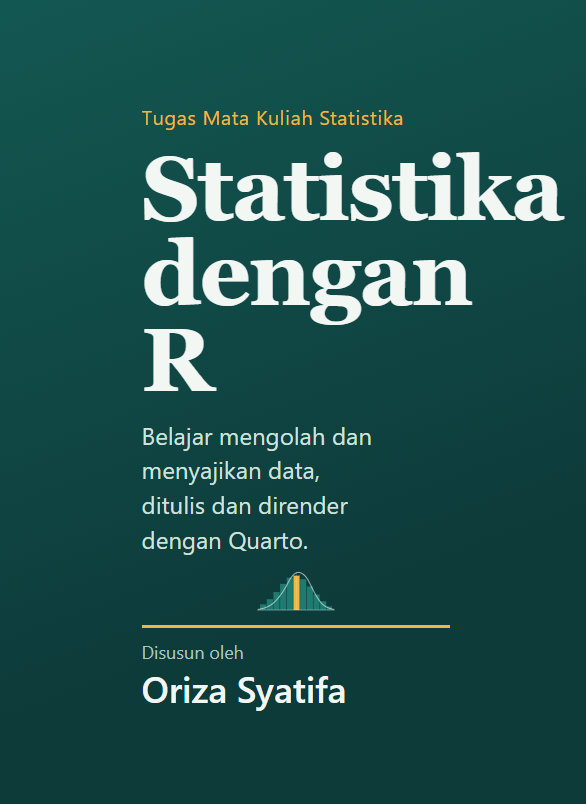
\includegraphics[height=\paperheight,keepaspectratio]{images/Cover.png}
  \end{titlepage}
  \restoregeometry
}

\makeatletter
\@ifpackageloaded{bookmark}{}{\usepackage{bookmark}}
\makeatother
\makeatletter
\@ifpackageloaded{caption}{}{\usepackage{caption}}
\AtBeginDocument{%
\ifdefined\contentsname
  \renewcommand*\contentsname{Daftar Isi}
\else
  \newcommand\contentsname{Daftar Isi}
\fi
\ifdefined\listfigurename
  \renewcommand*\listfigurename{Daftar Gambar}
\else
  \newcommand\listfigurename{Daftar Gambar}
\fi
\ifdefined\listtablename
  \renewcommand*\listtablename{Daftar Tabel}
\else
  \newcommand\listtablename{Daftar Tabel}
\fi
\ifdefined\figurename
  \renewcommand*\figurename{Gambar}
\else
  \newcommand\figurename{Gambar}
\fi
\ifdefined\tablename
  \renewcommand*\tablename{Tabel}
\else
  \newcommand\tablename{Tabel}
\fi
}
\@ifpackageloaded{float}{}{\usepackage{float}}
\floatstyle{ruled}
\@ifundefined{c@chapter}{\newfloat{codelisting}{h}{lop}}{\newfloat{codelisting}{h}{lop}[chapter]}
\floatname{codelisting}{Daftar}
\newcommand*\listoflistings{\listof{codelisting}{Daftar Daftar}}
\makeatother
\makeatletter
\makeatother
\makeatletter
\@ifpackageloaded{caption}{}{\usepackage{caption}}
\@ifpackageloaded{subcaption}{}{\usepackage{subcaption}}
\makeatother
\usepackage{bookmark}
\IfFileExists{xurl.sty}{\usepackage{xurl}}{} % add URL line breaks if available
\urlstyle{same}
% fallback for those not using the hyperref driver hyperxmp:
\makeatletter
\@ifundefined{xmpquote}{\newcommand{\xmpquote}[1]{#1}}{}
\makeatother
\hypersetup{
  pdftitle={Quarto Template},
  pdfauthor={Oriza Syatifa},
  pdflang={id},
  hidelinks,
  pdfcreator={LaTeX via pandoc}}


\title{Quarto Template}
\author{Oriza Syatifa}
\date{2026-11-25}
\begin{document}
\frontmatter
\maketitle

\renewcommand*\contentsname{Daftar Isi}
{
\setcounter{tocdepth}{2}
\tableofcontents
}

\mainmatter
\bookmarksetup{startatroot}

\chapter*{Kata Pengantar}\label{kata-pengantar}
\addcontentsline{toc}{chapter}{Kata Pengantar}

\markboth{Kata Pengantar}{Kata Pengantar}

Dengan mengucap syukur kepada Tuhan Yang Maha Esa, saya sangat senang
dapat mempersembahkan eBook \textbf{``Quarto Template''} kepada para
pembaca dan pengguna. eBook ini disusun sebagai panduan praktis untuk
membantu mahasiswa, dosen, peneliti, serta praktisi dalam memanfaatkan
Quarto sebagai salah satu perangkat untuk menyusun, mengelola, dan
menerbitkan dokumen secara profesional.

Quarto merupakan perangkat \emph{open-source scientific and technical
publishing} yang memungkinkan pengguna mengintegrasikan teks, kode
pemrograman, hasil analisis, visualisasi data, serta berbagai elemen
pendukung lainnya ke dalam satu dokumen. Dengan Quarto, proses penulisan
dan publikasi dapat dilakukan secara lebih terstruktur, reproducible,
dan efisien dalam berbagai format keluaran, seperti HTML, PDF, Microsoft
Word, serta format publikasi lainnya.

Contoh sitasi: tuliskan \texttt{{[}@xie2015{]}} untuk merujuk entri
\texttt{xie2015} di \texttt{references/book.bib}. Pada hasil render,
sitasinya tampil seperti ini \citeproc{ref-xie2015}{{[}1{]}}.

Melalui eBook ini, pembaca akan diperkenalkan pada penggunaan template
Quarto, mulai dari pengenalan struktur proyek, pengaturan konfigurasi,
penulisan dokumen menggunakan Markdown, integrasi kode pemrograman,
pengelolaan referensi, hingga proses \emph{rendering} menjadi dokumen
yang siap digunakan dan dipublikasikan.

Materi disusun secara bertahap agar mudah dipahami dan dipraktikkan,
termasuk oleh pengguna yang baru pertama kali mengenal Quarto. Template
dan contoh yang disajikan diharapkan dapat menjadi referensi dalam
mengembangkan berbagai kebutuhan dokumentasi akademik, laporan
penelitian, modul pembelajaran, buku elektronik, maupun publikasi
berbasis data.

Saya berharap eBook ini dapat memberikan manfaat nyata dalam mendukung
peningkatan literasi digital, produktivitas akademik, dan penerapan
praktik penulisan ilmiah yang modern. Lebih dari sekadar panduan teknis,
eBook ini diharapkan dapat mendorong pembaca untuk mengeksplorasi
berbagai kemampuan Quarto dan mengembangkan template sesuai dengan
kebutuhan masing-masing.

Saya menyadari bahwa eBook ini masih memiliki ruang untuk penyempurnaan.
Oleh karena itu, kritik, saran, dan masukan dari para pembaca sangat
diharapkan sebagai bahan evaluasi untuk pengembangan edisi berikutnya.

Akhir kata, semoga eBook ini dapat menjadi referensi yang bermanfaat dan
memberikan kontribusi positif bagi dunia pendidikan, penelitian, dan
pengembangan ilmu pengetahuan.

\textbf{Oriza Syatifa}\\
Penulis

\section*{Penulis}\label{penulis}
\addcontentsline{toc}{section}{Penulis}

\markright{Penulis}

\begin{figure}[H]

{\centering 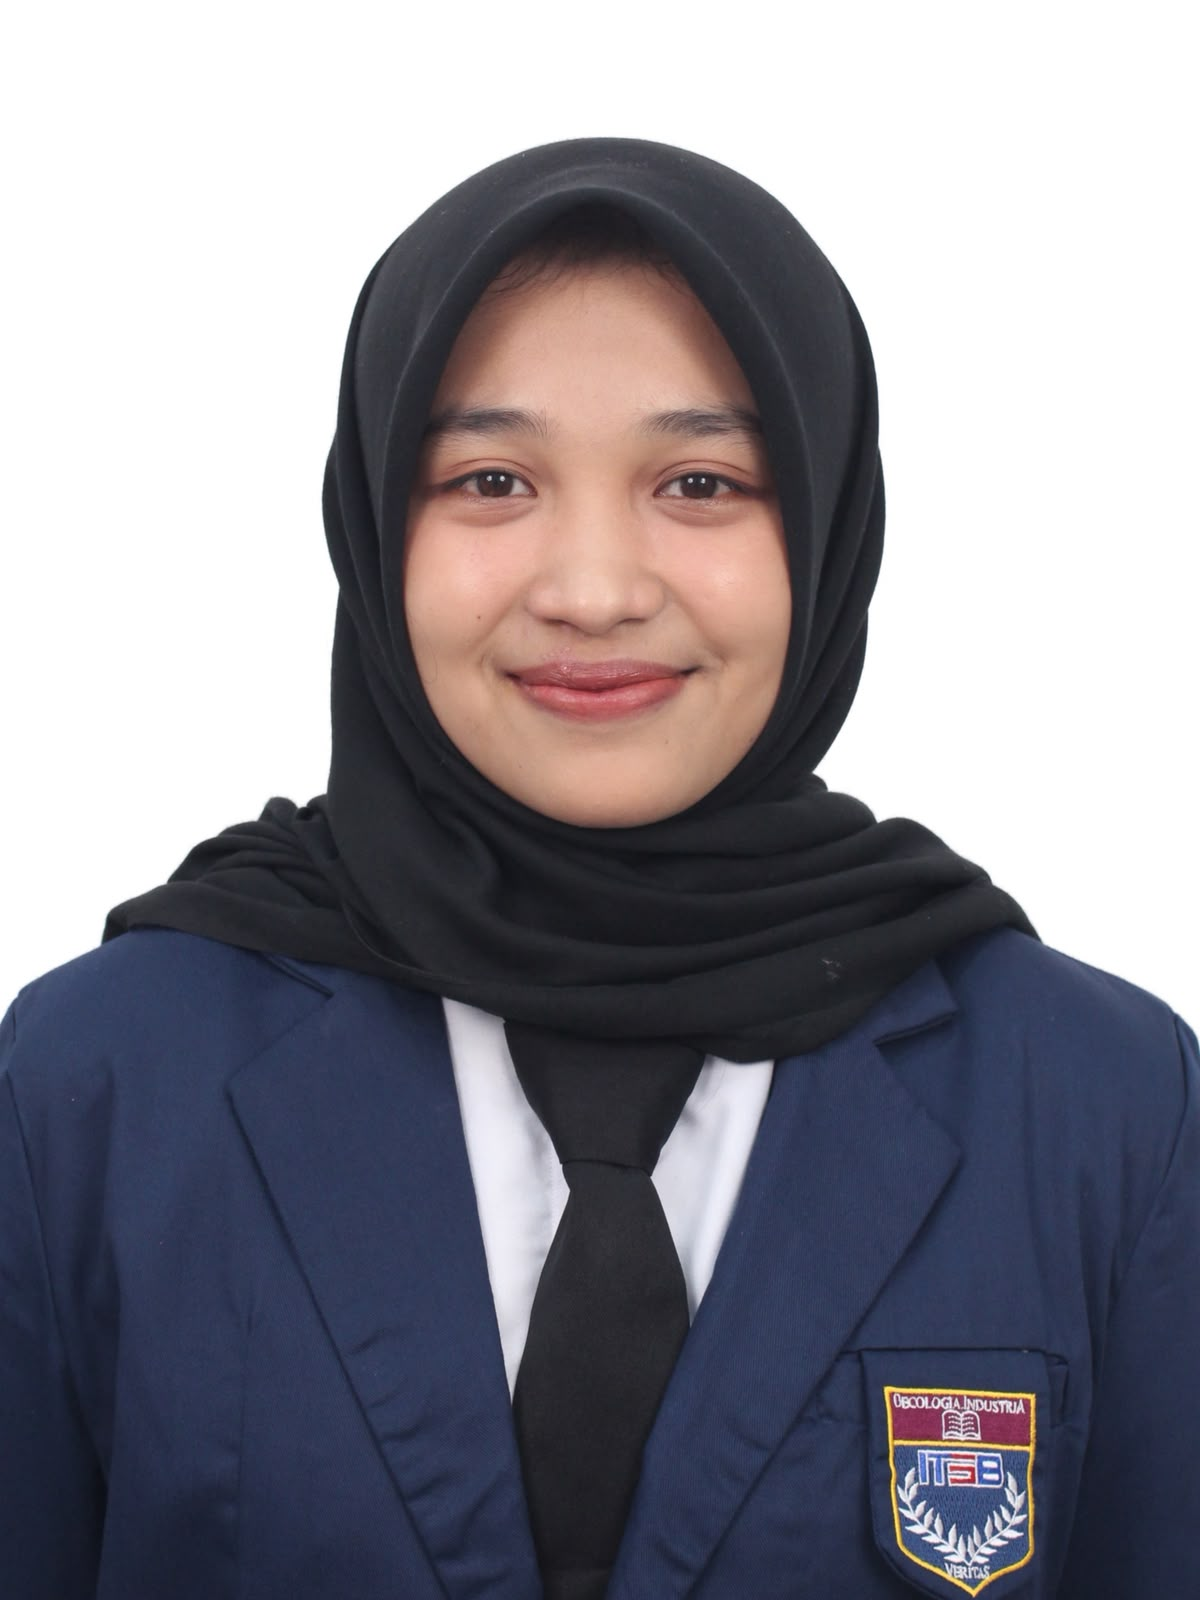
\includegraphics[width=1.5in,height=\textheight,keepaspectratio]{images/author/orizaa.jpeg}

}

\caption{Foto  Siregar, M.Sc.}

\end{figure}%

\textbf{\href{www.linkedin.com/in/oriza-syatifa-46826a440}{Oriza Syatifa}} bekerja sebagai Dosen di Prodi Sains Data Institut
Teknologi Sains Bandung. Beliau adalah meraih gelar Magister-nya dari
Departemen Matematika Terapan (Applied Mathematics) National Sun Yat Sen
University, Taiwan. Selain mengajar beliau juga pernah bekerja sebagai
\textbf{Data Scientist Freelance} di perusahaan-perusahaan ternama
seperti \href{https://www.jne.co.id/id/beranda}{JNE},
\href{https://www.samoragroup.co.id/home/en}{Samora Group},
\href{https://www.pertamina.com/}{Pertamina}, dan saat ini masih aktif
sebagai \textbf{Data Scientist Freelance} di
\href{PT.\%20Green\%20City\%20Traffic}{PT. Green City Traffic}. Beliau
memiliki antusiasme khusus dalam mengerjakan proyek (mengajar) Big Data
Analytics, Machine Learning, Optimisasi, dan Analisis Time Series di
bidang keuangan dan investasi. Keahlian utama yang dimilikinya adalah
bahasa pemrograman Statistik seperti R Studio dan Python. Beliau juga
sudah terbiasa dalam mengaplikasikan sistem basis data MySQL/NoSQL untuk
manajemen data, serta mahir dalam menggunakan tools Big Data seperti
Spark dan Hadoop. Beberapa project beliau dapat dilihat di link berikut:
\href{https://rpubs.com/dsciencelabs}{Rpubs},
\href{https://github.com/dsciencelabs}{Github},
\href{https://dsciencelabs.github.io/web/index.html}{Website}, dan
\href{https://www.kaggle.com/baktisiregar/code}{Kaggle}.

\section*{Ucapan Terima Kasih}\label{ucapan-terima-kasih}
\addcontentsline{toc}{section}{Ucapan Terima Kasih}

\markright{Ucapan Terima Kasih}

Proses penulisan Tempate eBook ini tidak terlepas dari dukungan berbagai
pihak. Saya ingin mengucapkan terima kasih kepada:

\begin{itemize}
\tightlist
\item
  \textbf{Keluarga} yang selalu memberikan dukungan moral dan semangat
  tanpa henti.
\item
  \textbf{Rekan-rekan dan Kolaborator} yang telah memberikan masukan,
  saran, dan kritik yang konstruktif.
\item
  Institusi dan Organisasi, Khususnya
  \textbf{\href{https://itsb.ac.id/}{ITSB}} yang telah menyediakan
  sumber daya dan fasilitas yang diperlukan selama proses penelitian dan
  penulisan.
\end{itemize}

Saya berharap Template eBook ini dapat menjadi referensi yang bermanfaat
dan memberikan inspirasi serta pengetahuan baru bagi pembaca. Semoga
Ebook ini dapat memenuhi ekspektasi dan kebutuhan para pembaca dan
semoga ilmu yang disampaikan dapat bermanfaat bagi semua.

\section*{Masukan \& Saran}\label{masukan-saran}
\addcontentsline{toc}{section}{Masukan \& Saran}

\markright{Masukan \& Saran}

Semua masukan dan tanggapan Anda sangat berarti bagi kami untuk
memperbaiki Ebook Quarto Template ini kedepannya. Bagi para
pembaca/pengguna yang ingin menyampaikan masukan dan tanggapan,
dipersilahkan melalui kontak dibawah ini!

\textbf{Email:} dsciencelabs@outlook.com

\bookmarksetup{startatroot}

\chapter{Distribusi Sampling}\label{distribusi-sampling}

\section{Pendahuluan}\label{pendahuluan}

\bookmarksetup{startatroot}

\chapter{Hypothesis Testing}\label{hypothesis-testing}

\section{Pendahuluan}\label{pendahuluan-1}

\bookmarksetup{startatroot}

\chapter{Bab3}\label{bab3}

\section{Praktikum}\label{praktikum}

\bookmarksetup{startatroot}

\chapter*{Referensi}\label{referensi}
\addcontentsline{toc}{chapter}{Referensi}

\markboth{Referensi}{Referensi}

\protect\phantomsection\label{refs}
\begin{CSLReferences}{0}{0}
\bibitem[\citeproctext]{ref-xie2015}
\CSLLeftMargin{{[}1{]} }%
\CSLRightInline{Y. Xie, \emph{\href{http://yihui.name/knitr/}{Dynamic
Documents with {R} and knitr}}, 2nd ed. Boca Raton, Florida: Chapman;
Hall/CRC, 2015.}

\end{CSLReferences}


\backmatter


\end{document}
